
% Default to the notebook output style

    


% Inherit from the specified cell style.




    
\documentclass[11pt]{article}

    
    
    \usepackage[T1]{fontenc}
    % Nicer default font (+ math font) than Computer Modern for most use cases
    \usepackage{mathpazo}

    % Basic figure setup, for now with no caption control since it's done
    % automatically by Pandoc (which extracts ![](path) syntax from Markdown).
    \usepackage{graphicx}
    % We will generate all images so they have a width \maxwidth. This means
    % that they will get their normal width if they fit onto the page, but
    % are scaled down if they would overflow the margins.
    \makeatletter
    \def\maxwidth{\ifdim\Gin@nat@width>\linewidth\linewidth
    \else\Gin@nat@width\fi}
    \makeatother
    \let\Oldincludegraphics\includegraphics
    % Set max figure width to be 80% of text width, for now hardcoded.
    \renewcommand{\includegraphics}[1]{\Oldincludegraphics[width=.8\maxwidth]{#1}}
    % Ensure that by default, figures have no caption (until we provide a
    % proper Figure object with a Caption API and a way to capture that
    % in the conversion process - todo).
    \usepackage{caption}
    \DeclareCaptionLabelFormat{nolabel}{}
    \captionsetup{labelformat=nolabel}

    \usepackage{adjustbox} % Used to constrain images to a maximum size 
    \usepackage{xcolor} % Allow colors to be defined
    \usepackage{enumerate} % Needed for markdown enumerations to work
    \usepackage{geometry} % Used to adjust the document margins
    \usepackage{amsmath} % Equations
    \usepackage{amssymb} % Equations
    \usepackage{textcomp} % defines textquotesingle
    % Hack from http://tex.stackexchange.com/a/47451/13684:
    \AtBeginDocument{%
        \def\PYZsq{\textquotesingle}% Upright quotes in Pygmentized code
    }
    \usepackage{upquote} % Upright quotes for verbatim code
    \usepackage{eurosym} % defines \euro
    \usepackage[mathletters]{ucs} % Extended unicode (utf-8) support
    \usepackage[utf8x]{inputenc} % Allow utf-8 characters in the tex document
    \usepackage{fancyvrb} % verbatim replacement that allows latex
    \usepackage{grffile} % extends the file name processing of package graphics 
                         % to support a larger range 
    % The hyperref package gives us a pdf with properly built
    % internal navigation ('pdf bookmarks' for the table of contents,
    % internal cross-reference links, web links for URLs, etc.)
    \usepackage{hyperref}
    \usepackage{longtable} % longtable support required by pandoc >1.10
    \usepackage{booktabs}  % table support for pandoc > 1.12.2
    \usepackage[inline]{enumitem} % IRkernel/repr support (it uses the enumerate* environment)
    \usepackage[normalem]{ulem} % ulem is needed to support strikethroughs (\sout)
                                % normalem makes italics be italics, not underlines
    

    
    
    % Colors for the hyperref package
    \definecolor{urlcolor}{rgb}{0,.145,.698}
    \definecolor{linkcolor}{rgb}{.71,0.21,0.01}
    \definecolor{citecolor}{rgb}{.12,.54,.11}

    % ANSI colors
    \definecolor{ansi-black}{HTML}{3E424D}
    \definecolor{ansi-black-intense}{HTML}{282C36}
    \definecolor{ansi-red}{HTML}{E75C58}
    \definecolor{ansi-red-intense}{HTML}{B22B31}
    \definecolor{ansi-green}{HTML}{00A250}
    \definecolor{ansi-green-intense}{HTML}{007427}
    \definecolor{ansi-yellow}{HTML}{DDB62B}
    \definecolor{ansi-yellow-intense}{HTML}{B27D12}
    \definecolor{ansi-blue}{HTML}{208FFB}
    \definecolor{ansi-blue-intense}{HTML}{0065CA}
    \definecolor{ansi-magenta}{HTML}{D160C4}
    \definecolor{ansi-magenta-intense}{HTML}{A03196}
    \definecolor{ansi-cyan}{HTML}{60C6C8}
    \definecolor{ansi-cyan-intense}{HTML}{258F8F}
    \definecolor{ansi-white}{HTML}{C5C1B4}
    \definecolor{ansi-white-intense}{HTML}{A1A6B2}

    % commands and environments needed by pandoc snippets
    % extracted from the output of `pandoc -s`
    \providecommand{\tightlist}{%
      \setlength{\itemsep}{0pt}\setlength{\parskip}{0pt}}
    \DefineVerbatimEnvironment{Highlighting}{Verbatim}{commandchars=\\\{\}}
    % Add ',fontsize=\small' for more characters per line
    \newenvironment{Shaded}{}{}
    \newcommand{\KeywordTok}[1]{\textcolor[rgb]{0.00,0.44,0.13}{\textbf{{#1}}}}
    \newcommand{\DataTypeTok}[1]{\textcolor[rgb]{0.56,0.13,0.00}{{#1}}}
    \newcommand{\DecValTok}[1]{\textcolor[rgb]{0.25,0.63,0.44}{{#1}}}
    \newcommand{\BaseNTok}[1]{\textcolor[rgb]{0.25,0.63,0.44}{{#1}}}
    \newcommand{\FloatTok}[1]{\textcolor[rgb]{0.25,0.63,0.44}{{#1}}}
    \newcommand{\CharTok}[1]{\textcolor[rgb]{0.25,0.44,0.63}{{#1}}}
    \newcommand{\StringTok}[1]{\textcolor[rgb]{0.25,0.44,0.63}{{#1}}}
    \newcommand{\CommentTok}[1]{\textcolor[rgb]{0.38,0.63,0.69}{\textit{{#1}}}}
    \newcommand{\OtherTok}[1]{\textcolor[rgb]{0.00,0.44,0.13}{{#1}}}
    \newcommand{\AlertTok}[1]{\textcolor[rgb]{1.00,0.00,0.00}{\textbf{{#1}}}}
    \newcommand{\FunctionTok}[1]{\textcolor[rgb]{0.02,0.16,0.49}{{#1}}}
    \newcommand{\RegionMarkerTok}[1]{{#1}}
    \newcommand{\ErrorTok}[1]{\textcolor[rgb]{1.00,0.00,0.00}{\textbf{{#1}}}}
    \newcommand{\NormalTok}[1]{{#1}}
    
    % Additional commands for more recent versions of Pandoc
    \newcommand{\ConstantTok}[1]{\textcolor[rgb]{0.53,0.00,0.00}{{#1}}}
    \newcommand{\SpecialCharTok}[1]{\textcolor[rgb]{0.25,0.44,0.63}{{#1}}}
    \newcommand{\VerbatimStringTok}[1]{\textcolor[rgb]{0.25,0.44,0.63}{{#1}}}
    \newcommand{\SpecialStringTok}[1]{\textcolor[rgb]{0.73,0.40,0.53}{{#1}}}
    \newcommand{\ImportTok}[1]{{#1}}
    \newcommand{\DocumentationTok}[1]{\textcolor[rgb]{0.73,0.13,0.13}{\textit{{#1}}}}
    \newcommand{\AnnotationTok}[1]{\textcolor[rgb]{0.38,0.63,0.69}{\textbf{\textit{{#1}}}}}
    \newcommand{\CommentVarTok}[1]{\textcolor[rgb]{0.38,0.63,0.69}{\textbf{\textit{{#1}}}}}
    \newcommand{\VariableTok}[1]{\textcolor[rgb]{0.10,0.09,0.49}{{#1}}}
    \newcommand{\ControlFlowTok}[1]{\textcolor[rgb]{0.00,0.44,0.13}{\textbf{{#1}}}}
    \newcommand{\OperatorTok}[1]{\textcolor[rgb]{0.40,0.40,0.40}{{#1}}}
    \newcommand{\BuiltInTok}[1]{{#1}}
    \newcommand{\ExtensionTok}[1]{{#1}}
    \newcommand{\PreprocessorTok}[1]{\textcolor[rgb]{0.74,0.48,0.00}{{#1}}}
    \newcommand{\AttributeTok}[1]{\textcolor[rgb]{0.49,0.56,0.16}{{#1}}}
    \newcommand{\InformationTok}[1]{\textcolor[rgb]{0.38,0.63,0.69}{\textbf{\textit{{#1}}}}}
    \newcommand{\WarningTok}[1]{\textcolor[rgb]{0.38,0.63,0.69}{\textbf{\textit{{#1}}}}}
    
    
    % Define a nice break command that doesn't care if a line doesn't already
    % exist.
    \def\br{\hspace*{\fill} \\* }
    % Math Jax compatability definitions
    \def\gt{>}
    \def\lt{<}
    % Document parameters
    \title{Untitled1}
    
    
    

    % Pygments definitions
    
\makeatletter
\def\PY@reset{\let\PY@it=\relax \let\PY@bf=\relax%
    \let\PY@ul=\relax \let\PY@tc=\relax%
    \let\PY@bc=\relax \let\PY@ff=\relax}
\def\PY@tok#1{\csname PY@tok@#1\endcsname}
\def\PY@toks#1+{\ifx\relax#1\empty\else%
    \PY@tok{#1}\expandafter\PY@toks\fi}
\def\PY@do#1{\PY@bc{\PY@tc{\PY@ul{%
    \PY@it{\PY@bf{\PY@ff{#1}}}}}}}
\def\PY#1#2{\PY@reset\PY@toks#1+\relax+\PY@do{#2}}

\expandafter\def\csname PY@tok@w\endcsname{\def\PY@tc##1{\textcolor[rgb]{0.73,0.73,0.73}{##1}}}
\expandafter\def\csname PY@tok@c\endcsname{\let\PY@it=\textit\def\PY@tc##1{\textcolor[rgb]{0.25,0.50,0.50}{##1}}}
\expandafter\def\csname PY@tok@cp\endcsname{\def\PY@tc##1{\textcolor[rgb]{0.74,0.48,0.00}{##1}}}
\expandafter\def\csname PY@tok@k\endcsname{\let\PY@bf=\textbf\def\PY@tc##1{\textcolor[rgb]{0.00,0.50,0.00}{##1}}}
\expandafter\def\csname PY@tok@kp\endcsname{\def\PY@tc##1{\textcolor[rgb]{0.00,0.50,0.00}{##1}}}
\expandafter\def\csname PY@tok@kt\endcsname{\def\PY@tc##1{\textcolor[rgb]{0.69,0.00,0.25}{##1}}}
\expandafter\def\csname PY@tok@o\endcsname{\def\PY@tc##1{\textcolor[rgb]{0.40,0.40,0.40}{##1}}}
\expandafter\def\csname PY@tok@ow\endcsname{\let\PY@bf=\textbf\def\PY@tc##1{\textcolor[rgb]{0.67,0.13,1.00}{##1}}}
\expandafter\def\csname PY@tok@nb\endcsname{\def\PY@tc##1{\textcolor[rgb]{0.00,0.50,0.00}{##1}}}
\expandafter\def\csname PY@tok@nf\endcsname{\def\PY@tc##1{\textcolor[rgb]{0.00,0.00,1.00}{##1}}}
\expandafter\def\csname PY@tok@nc\endcsname{\let\PY@bf=\textbf\def\PY@tc##1{\textcolor[rgb]{0.00,0.00,1.00}{##1}}}
\expandafter\def\csname PY@tok@nn\endcsname{\let\PY@bf=\textbf\def\PY@tc##1{\textcolor[rgb]{0.00,0.00,1.00}{##1}}}
\expandafter\def\csname PY@tok@ne\endcsname{\let\PY@bf=\textbf\def\PY@tc##1{\textcolor[rgb]{0.82,0.25,0.23}{##1}}}
\expandafter\def\csname PY@tok@nv\endcsname{\def\PY@tc##1{\textcolor[rgb]{0.10,0.09,0.49}{##1}}}
\expandafter\def\csname PY@tok@no\endcsname{\def\PY@tc##1{\textcolor[rgb]{0.53,0.00,0.00}{##1}}}
\expandafter\def\csname PY@tok@nl\endcsname{\def\PY@tc##1{\textcolor[rgb]{0.63,0.63,0.00}{##1}}}
\expandafter\def\csname PY@tok@ni\endcsname{\let\PY@bf=\textbf\def\PY@tc##1{\textcolor[rgb]{0.60,0.60,0.60}{##1}}}
\expandafter\def\csname PY@tok@na\endcsname{\def\PY@tc##1{\textcolor[rgb]{0.49,0.56,0.16}{##1}}}
\expandafter\def\csname PY@tok@nt\endcsname{\let\PY@bf=\textbf\def\PY@tc##1{\textcolor[rgb]{0.00,0.50,0.00}{##1}}}
\expandafter\def\csname PY@tok@nd\endcsname{\def\PY@tc##1{\textcolor[rgb]{0.67,0.13,1.00}{##1}}}
\expandafter\def\csname PY@tok@s\endcsname{\def\PY@tc##1{\textcolor[rgb]{0.73,0.13,0.13}{##1}}}
\expandafter\def\csname PY@tok@sd\endcsname{\let\PY@it=\textit\def\PY@tc##1{\textcolor[rgb]{0.73,0.13,0.13}{##1}}}
\expandafter\def\csname PY@tok@si\endcsname{\let\PY@bf=\textbf\def\PY@tc##1{\textcolor[rgb]{0.73,0.40,0.53}{##1}}}
\expandafter\def\csname PY@tok@se\endcsname{\let\PY@bf=\textbf\def\PY@tc##1{\textcolor[rgb]{0.73,0.40,0.13}{##1}}}
\expandafter\def\csname PY@tok@sr\endcsname{\def\PY@tc##1{\textcolor[rgb]{0.73,0.40,0.53}{##1}}}
\expandafter\def\csname PY@tok@ss\endcsname{\def\PY@tc##1{\textcolor[rgb]{0.10,0.09,0.49}{##1}}}
\expandafter\def\csname PY@tok@sx\endcsname{\def\PY@tc##1{\textcolor[rgb]{0.00,0.50,0.00}{##1}}}
\expandafter\def\csname PY@tok@m\endcsname{\def\PY@tc##1{\textcolor[rgb]{0.40,0.40,0.40}{##1}}}
\expandafter\def\csname PY@tok@gh\endcsname{\let\PY@bf=\textbf\def\PY@tc##1{\textcolor[rgb]{0.00,0.00,0.50}{##1}}}
\expandafter\def\csname PY@tok@gu\endcsname{\let\PY@bf=\textbf\def\PY@tc##1{\textcolor[rgb]{0.50,0.00,0.50}{##1}}}
\expandafter\def\csname PY@tok@gd\endcsname{\def\PY@tc##1{\textcolor[rgb]{0.63,0.00,0.00}{##1}}}
\expandafter\def\csname PY@tok@gi\endcsname{\def\PY@tc##1{\textcolor[rgb]{0.00,0.63,0.00}{##1}}}
\expandafter\def\csname PY@tok@gr\endcsname{\def\PY@tc##1{\textcolor[rgb]{1.00,0.00,0.00}{##1}}}
\expandafter\def\csname PY@tok@ge\endcsname{\let\PY@it=\textit}
\expandafter\def\csname PY@tok@gs\endcsname{\let\PY@bf=\textbf}
\expandafter\def\csname PY@tok@gp\endcsname{\let\PY@bf=\textbf\def\PY@tc##1{\textcolor[rgb]{0.00,0.00,0.50}{##1}}}
\expandafter\def\csname PY@tok@go\endcsname{\def\PY@tc##1{\textcolor[rgb]{0.53,0.53,0.53}{##1}}}
\expandafter\def\csname PY@tok@gt\endcsname{\def\PY@tc##1{\textcolor[rgb]{0.00,0.27,0.87}{##1}}}
\expandafter\def\csname PY@tok@err\endcsname{\def\PY@bc##1{\setlength{\fboxsep}{0pt}\fcolorbox[rgb]{1.00,0.00,0.00}{1,1,1}{\strut ##1}}}
\expandafter\def\csname PY@tok@kc\endcsname{\let\PY@bf=\textbf\def\PY@tc##1{\textcolor[rgb]{0.00,0.50,0.00}{##1}}}
\expandafter\def\csname PY@tok@kd\endcsname{\let\PY@bf=\textbf\def\PY@tc##1{\textcolor[rgb]{0.00,0.50,0.00}{##1}}}
\expandafter\def\csname PY@tok@kn\endcsname{\let\PY@bf=\textbf\def\PY@tc##1{\textcolor[rgb]{0.00,0.50,0.00}{##1}}}
\expandafter\def\csname PY@tok@kr\endcsname{\let\PY@bf=\textbf\def\PY@tc##1{\textcolor[rgb]{0.00,0.50,0.00}{##1}}}
\expandafter\def\csname PY@tok@bp\endcsname{\def\PY@tc##1{\textcolor[rgb]{0.00,0.50,0.00}{##1}}}
\expandafter\def\csname PY@tok@fm\endcsname{\def\PY@tc##1{\textcolor[rgb]{0.00,0.00,1.00}{##1}}}
\expandafter\def\csname PY@tok@vc\endcsname{\def\PY@tc##1{\textcolor[rgb]{0.10,0.09,0.49}{##1}}}
\expandafter\def\csname PY@tok@vg\endcsname{\def\PY@tc##1{\textcolor[rgb]{0.10,0.09,0.49}{##1}}}
\expandafter\def\csname PY@tok@vi\endcsname{\def\PY@tc##1{\textcolor[rgb]{0.10,0.09,0.49}{##1}}}
\expandafter\def\csname PY@tok@vm\endcsname{\def\PY@tc##1{\textcolor[rgb]{0.10,0.09,0.49}{##1}}}
\expandafter\def\csname PY@tok@sa\endcsname{\def\PY@tc##1{\textcolor[rgb]{0.73,0.13,0.13}{##1}}}
\expandafter\def\csname PY@tok@sb\endcsname{\def\PY@tc##1{\textcolor[rgb]{0.73,0.13,0.13}{##1}}}
\expandafter\def\csname PY@tok@sc\endcsname{\def\PY@tc##1{\textcolor[rgb]{0.73,0.13,0.13}{##1}}}
\expandafter\def\csname PY@tok@dl\endcsname{\def\PY@tc##1{\textcolor[rgb]{0.73,0.13,0.13}{##1}}}
\expandafter\def\csname PY@tok@s2\endcsname{\def\PY@tc##1{\textcolor[rgb]{0.73,0.13,0.13}{##1}}}
\expandafter\def\csname PY@tok@sh\endcsname{\def\PY@tc##1{\textcolor[rgb]{0.73,0.13,0.13}{##1}}}
\expandafter\def\csname PY@tok@s1\endcsname{\def\PY@tc##1{\textcolor[rgb]{0.73,0.13,0.13}{##1}}}
\expandafter\def\csname PY@tok@mb\endcsname{\def\PY@tc##1{\textcolor[rgb]{0.40,0.40,0.40}{##1}}}
\expandafter\def\csname PY@tok@mf\endcsname{\def\PY@tc##1{\textcolor[rgb]{0.40,0.40,0.40}{##1}}}
\expandafter\def\csname PY@tok@mh\endcsname{\def\PY@tc##1{\textcolor[rgb]{0.40,0.40,0.40}{##1}}}
\expandafter\def\csname PY@tok@mi\endcsname{\def\PY@tc##1{\textcolor[rgb]{0.40,0.40,0.40}{##1}}}
\expandafter\def\csname PY@tok@il\endcsname{\def\PY@tc##1{\textcolor[rgb]{0.40,0.40,0.40}{##1}}}
\expandafter\def\csname PY@tok@mo\endcsname{\def\PY@tc##1{\textcolor[rgb]{0.40,0.40,0.40}{##1}}}
\expandafter\def\csname PY@tok@ch\endcsname{\let\PY@it=\textit\def\PY@tc##1{\textcolor[rgb]{0.25,0.50,0.50}{##1}}}
\expandafter\def\csname PY@tok@cm\endcsname{\let\PY@it=\textit\def\PY@tc##1{\textcolor[rgb]{0.25,0.50,0.50}{##1}}}
\expandafter\def\csname PY@tok@cpf\endcsname{\let\PY@it=\textit\def\PY@tc##1{\textcolor[rgb]{0.25,0.50,0.50}{##1}}}
\expandafter\def\csname PY@tok@c1\endcsname{\let\PY@it=\textit\def\PY@tc##1{\textcolor[rgb]{0.25,0.50,0.50}{##1}}}
\expandafter\def\csname PY@tok@cs\endcsname{\let\PY@it=\textit\def\PY@tc##1{\textcolor[rgb]{0.25,0.50,0.50}{##1}}}

\def\PYZbs{\char`\\}
\def\PYZus{\char`\_}
\def\PYZob{\char`\{}
\def\PYZcb{\char`\}}
\def\PYZca{\char`\^}
\def\PYZam{\char`\&}
\def\PYZlt{\char`\<}
\def\PYZgt{\char`\>}
\def\PYZsh{\char`\#}
\def\PYZpc{\char`\%}
\def\PYZdl{\char`\$}
\def\PYZhy{\char`\-}
\def\PYZsq{\char`\'}
\def\PYZdq{\char`\"}
\def\PYZti{\char`\~}
% for compatibility with earlier versions
\def\PYZat{@}
\def\PYZlb{[}
\def\PYZrb{]}
\makeatother


    % Exact colors from NB
    \definecolor{incolor}{rgb}{0.0, 0.0, 0.5}
    \definecolor{outcolor}{rgb}{0.545, 0.0, 0.0}



    
    % Prevent overflowing lines due to hard-to-break entities
    \sloppy 
    % Setup hyperref package
    \hypersetup{
      breaklinks=true,  % so long urls are correctly broken across lines
      colorlinks=true,
      urlcolor=urlcolor,
      linkcolor=linkcolor,
      citecolor=citecolor,
      }
    % Slightly bigger margins than the latex defaults
    
    \geometry{verbose,tmargin=1in,bmargin=1in,lmargin=1in,rmargin=1in}
    
    

    \begin{document}
    
    
    \maketitle
    
    

    
    \subsection{Milestone Capstone:}\label{milestone-capstone}

\section{Utilizing Meteorological Data with Supervised Learning to
Predict Snowfall Amounts at Ski
Resort}\label{utilizing-meteorological-data-with-supervised-learning-to-predict-snowfall-amounts-at-ski-resort}

\textbf{By Dustin Rapp}

\subsection{-\/-}\label{section}

\subsection{Introduction}\label{introduction}

\begin{center}\rule{0.5\linewidth}{\linethickness}\end{center}

Complex terrain in mountainous areas often make predicting snowfall
difficult with prognostic weather models - especially on specific slopes
or mountainsides where extremely localized air flows may complicate such
forecasts. With accurate snow forecasts, ski resorts can optimize their
snowfall making, grooming, and snow removal operations. An accurate
short term snowfall forecast, even for a small segment of the mountain
may likely assist a ski resort's operation. The goal of this study is to
get a glimpse into the potential of utilizing a supervised learning
techniques with freely available surface and meteorological data to
predict snowfall on a slope at Copper Mountain Ski Resort in Colorado.
Copper Mountain Ski Resort may be especially interested in such
predictive models because of the unique access to government funded
meteorological data being recorded near or onsite to their resort.

The purpose of this report is to discuss data to be utilized and make
general assessment regarding how well a supervised learning model might
perform .

\subsection{Data}\label{data}

The Copper Mountain ski resort is unique as there is an official SNOTEL
National Resources Conservation Service monitoring station the north
slope of Copper Mountain, where many popular ski runs are located.
SNOTEL is a telemetry automated system of snowpack and related climate
sensors in the Western United States. In addition to reporting hourly
snowfall amounts, it also records temperature. The Copper Mountain ski
resort is also has an Colorado Department of Transportation Automated
Weather Observing System (AWOS) which monitors a suite of hourly
variables near the top of Copper Mountain. Additionally, a National
Weather Service Automated Surface Observing Station (ASOS) is located in
Leadville, CO approximately 30 km to the northwest of Copper Mountain.
These three stations give a comprehensive meteorological dataset of
surface variables in the vicinity of the Copper Mountain Resort.
\textbf{Table 1-1} gives a listing of all surface level meteorological
variables by station. Hourly data for each station was downloaded for
years 2005-2017 from online sources. Data sources for each station are
found in \textbf{Table 2}.

A map showing the Copper Mountain SNOTEL site and the meteorological
sites used in this assessment is also shown in \textbf{Figure 1}

\begin{center}\rule{0.5\linewidth}{\linethickness}\end{center}

\textbf{Figure 1 - Map of Locations}

\begin{center}\rule{0.5\linewidth}{\linethickness}\end{center}

\textbf{Table 1 - Meteorological Variables by Station}

\begin{longtable}[]{@{}ccr@{}}
\toprule
SNOTEL & LXV ASOS & KCCU AWOS\tabularnewline
\midrule
\endhead
Temperature & Temperature & Temperature\tabularnewline
Snow Depth & Dewpoint & Dewpoint\tabularnewline
& Wind Speed & Wind Speed\tabularnewline
& Wind Direction & Wind Direction\tabularnewline
& Cloud Cover & Cloud Cover\tabularnewline
\bottomrule
\end{longtable}

\begin{center}\rule{0.5\linewidth}{\linethickness}\end{center}

\textbf{Table 2 - Sources of Meteorological Data.}

\begin{longtable}[]{@{}ll@{}}
\toprule
Station & Data Source\tabularnewline
\midrule
\endhead
SNOTEL & National Resources Conservation Service
(www.NRCS.gov)\tabularnewline
LXV ASOS & National Climatic Data Center - ISHD Lite format
(www.NCDC.gov)\tabularnewline
KCCU AWOS & National Climatic Data Center (ISHD format)
(www.NCDC.gov)\tabularnewline
\bottomrule
\end{longtable}

\subsection{Data and Wrangling
Cleaning}\label{data-and-wrangling-cleaning}

\subsubsection{Data Organization}\label{data-organization}

Hourly surface data from each station, downloaded, organized and
combined into a single timeseries dataframes with UTM timestamps.

The following cleanup steps were performed on this dataset:

\begin{itemize}
\tightlist
\item
  While the KCCU and KXLV datasets were already in UTM time, the NRCS
  dataset was in local time and required conversion to UTM.\\
\item
  The KCCU and KXLV datasets are in the Integrated Surface Hourly Data
  (ISHD) format and did require some manipulation (e.g. divided by 10)
  to get values into typical units.
\item
  Missing values (e.g. 9999 values) were translated to NaN values.
\item
  Missing data for all variables was linearly interpolated for time
  periods where 3 hours or less of data was missing.
\end{itemize}

The data was plotted to see if there were any extreme values warranting
removal. It was noted that some of the KCCU data (especially
temperature) did not demonstrate as much of a diurnal variation as the
KXLV station. These data are considered suspicious but were not removed
from the dataset. A more robust quality control of this dataset is
outside the scope of this prelimiaryn study, but should be considered
for future studies.

A small amount of anomalous data was observed in the SNOTEL snow depth
data and was removed. These physically unrealistic readings (e.g. spikes
in some of the snow depth data or snowdepth reports which occur when
temperatures did not support snowfall) were removed as well as extreme
negative values.

\subsubsection{Additional Calculations}\label{additional-calculations}

\textbf{Pressure}\\
Changes in pressure are often a predictive indicator of weather
conditions (i.e. pressure drops often accompany strong storm systems), a
twelve hour pressure change variable was added to the datset. This was
calculated by subtracting the 00:00 observation from the upcoming 12:00
observation.

\textbf{Snowfall}\\
As the SNOTEL data only includes snow depth data instead of snowfall
data, snowfall was calculated based on changes in snowdepth. Due to the
sensitivity of the SNOTEL snow depth measurement sensors to external
forces (e.g. debris, air pressure), snow depth data from the SNOTEL site
appeared noisy for smaller snowstorms (i.e. less then 3 inches). To
minimize the small scale perturbations found in the data, 12 hour
snowfall totals were estimated at 00:00 UTC and 12:00 UTC and only 12-hr
snowfall events where greater then or equal to 3 inches occurred were
considered a snowfall event. The snowfall data was then added to
meteorological dataframe.

Because only 00:00 and 12:00 snowfall observations were utilized in the
analysis, all variables in the meteorological dataframe were reduced
from hourly observations to twelve hour observations. A new dataframe
was created utilizing only 00:00 and 12:00 observations.

A table showing the total number of snowfall events, along with mean,
max, and standard deviation of snowfall for each year is found in
\textbf{Table 3}. A timeseries plot showing the snowdepth, along with
these snowfall events is found in \textbf{Figure 2}.

\begin{center}\rule{0.5\linewidth}{\linethickness}\end{center}

\textbf{Table 3 Statistics on Snowfall Events To be Used in Analysis}

\begin{longtable}[]{@{}lllllll@{}}
\toprule
\begin{minipage}[b]{0.06\columnwidth}\raggedright\strut
Year\strut
\end{minipage} & \begin{minipage}[b]{0.26\columnwidth}\raggedright\strut
Number 12hr Snowfall Events \textgreater{}=3\strut
\end{minipage} & \begin{minipage}[b]{0.06\columnwidth}\raggedright\strut
Mean\strut
\end{minipage} & \begin{minipage}[b]{0.08\columnwidth}\raggedright\strut
Median\strut
\end{minipage} & \begin{minipage}[b]{0.06\columnwidth}\raggedright\strut
Max\strut
\end{minipage} & \begin{minipage}[b]{0.16\columnwidth}\raggedright\strut
\%Missing SnowDepth\strut
\end{minipage} & \begin{minipage}[b]{0.13\columnwidth}\raggedright\strut
Std Deviation\strut
\end{minipage}\tabularnewline
\midrule
\endhead
\begin{minipage}[t]{0.06\columnwidth}\raggedright\strut
2006\strut
\end{minipage} & \begin{minipage}[t]{0.26\columnwidth}\raggedright\strut
26\strut
\end{minipage} & \begin{minipage}[t]{0.06\columnwidth}\raggedright\strut
4.8\strut
\end{minipage} & \begin{minipage}[t]{0.08\columnwidth}\raggedright\strut
4\strut
\end{minipage} & \begin{minipage}[t]{0.06\columnwidth}\raggedright\strut
11\strut
\end{minipage} & \begin{minipage}[t]{0.16\columnwidth}\raggedright\strut
0.69\strut
\end{minipage} & \begin{minipage}[t]{0.13\columnwidth}\raggedright\strut
1.87\strut
\end{minipage}\tabularnewline
\begin{minipage}[t]{0.06\columnwidth}\raggedright\strut
2007\strut
\end{minipage} & \begin{minipage}[t]{0.26\columnwidth}\raggedright\strut
29\strut
\end{minipage} & \begin{minipage}[t]{0.06\columnwidth}\raggedright\strut
3.9\strut
\end{minipage} & \begin{minipage}[t]{0.08\columnwidth}\raggedright\strut
3.3\strut
\end{minipage} & \begin{minipage}[t]{0.06\columnwidth}\raggedright\strut
6.5\strut
\end{minipage} & \begin{minipage}[t]{0.16\columnwidth}\raggedright\strut
0.69\strut
\end{minipage} & \begin{minipage}[t]{0.13\columnwidth}\raggedright\strut
1.17\strut
\end{minipage}\tabularnewline
\begin{minipage}[t]{0.06\columnwidth}\raggedright\strut
2008\strut
\end{minipage} & \begin{minipage}[t]{0.26\columnwidth}\raggedright\strut
27\strut
\end{minipage} & \begin{minipage}[t]{0.06\columnwidth}\raggedright\strut
4.5\strut
\end{minipage} & \begin{minipage}[t]{0.08\columnwidth}\raggedright\strut
3.7\strut
\end{minipage} & \begin{minipage}[t]{0.06\columnwidth}\raggedright\strut
8\strut
\end{minipage} & \begin{minipage}[t]{0.16\columnwidth}\raggedright\strut
0.69\strut
\end{minipage} & \begin{minipage}[t]{0.13\columnwidth}\raggedright\strut
1.85\strut
\end{minipage}\tabularnewline
\begin{minipage}[t]{0.06\columnwidth}\raggedright\strut
2009\strut
\end{minipage} & \begin{minipage}[t]{0.26\columnwidth}\raggedright\strut
27\strut
\end{minipage} & \begin{minipage}[t]{0.06\columnwidth}\raggedright\strut
4.3\strut
\end{minipage} & \begin{minipage}[t]{0.08\columnwidth}\raggedright\strut
4\strut
\end{minipage} & \begin{minipage}[t]{0.06\columnwidth}\raggedright\strut
13\strut
\end{minipage} & \begin{minipage}[t]{0.16\columnwidth}\raggedright\strut
0.69\strut
\end{minipage} & \begin{minipage}[t]{0.13\columnwidth}\raggedright\strut
1.92\strut
\end{minipage}\tabularnewline
\begin{minipage}[t]{0.06\columnwidth}\raggedright\strut
2010\strut
\end{minipage} & \begin{minipage}[t]{0.26\columnwidth}\raggedright\strut
30\strut
\end{minipage} & \begin{minipage}[t]{0.06\columnwidth}\raggedright\strut
4.6\strut
\end{minipage} & \begin{minipage}[t]{0.08\columnwidth}\raggedright\strut
4\strut
\end{minipage} & \begin{minipage}[t]{0.06\columnwidth}\raggedright\strut
9\strut
\end{minipage} & \begin{minipage}[t]{0.16\columnwidth}\raggedright\strut
0.69\strut
\end{minipage} & \begin{minipage}[t]{0.13\columnwidth}\raggedright\strut
1.75\strut
\end{minipage}\tabularnewline
\begin{minipage}[t]{0.06\columnwidth}\raggedright\strut
2011\strut
\end{minipage} & \begin{minipage}[t]{0.26\columnwidth}\raggedright\strut
32\strut
\end{minipage} & \begin{minipage}[t]{0.06\columnwidth}\raggedright\strut
4.3\strut
\end{minipage} & \begin{minipage}[t]{0.08\columnwidth}\raggedright\strut
4\strut
\end{minipage} & \begin{minipage}[t]{0.06\columnwidth}\raggedright\strut
7\strut
\end{minipage} & \begin{minipage}[t]{0.16\columnwidth}\raggedright\strut
0.69\strut
\end{minipage} & \begin{minipage}[t]{0.13\columnwidth}\raggedright\strut
1.38\strut
\end{minipage}\tabularnewline
\begin{minipage}[t]{0.06\columnwidth}\raggedright\strut
2012\strut
\end{minipage} & \begin{minipage}[t]{0.26\columnwidth}\raggedright\strut
14\strut
\end{minipage} & \begin{minipage}[t]{0.06\columnwidth}\raggedright\strut
5.1\strut
\end{minipage} & \begin{minipage}[t]{0.08\columnwidth}\raggedright\strut
4\strut
\end{minipage} & \begin{minipage}[t]{0.06\columnwidth}\raggedright\strut
10\strut
\end{minipage} & \begin{minipage}[t]{0.16\columnwidth}\raggedright\strut
0.69\strut
\end{minipage} & \begin{minipage}[t]{0.13\columnwidth}\raggedright\strut
2.29\strut
\end{minipage}\tabularnewline
\begin{minipage}[t]{0.06\columnwidth}\raggedright\strut
2013\strut
\end{minipage} & \begin{minipage}[t]{0.26\columnwidth}\raggedright\strut
32\strut
\end{minipage} & \begin{minipage}[t]{0.06\columnwidth}\raggedright\strut
4.3\strut
\end{minipage} & \begin{minipage}[t]{0.08\columnwidth}\raggedright\strut
4\strut
\end{minipage} & \begin{minipage}[t]{0.06\columnwidth}\raggedright\strut
12\strut
\end{minipage} & \begin{minipage}[t]{0.16\columnwidth}\raggedright\strut
0.69\strut
\end{minipage} & \begin{minipage}[t]{0.13\columnwidth}\raggedright\strut
1.78\strut
\end{minipage}\tabularnewline
\begin{minipage}[t]{0.06\columnwidth}\raggedright\strut
2015\strut
\end{minipage} & \begin{minipage}[t]{0.26\columnwidth}\raggedright\strut
23\strut
\end{minipage} & \begin{minipage}[t]{0.06\columnwidth}\raggedright\strut
4.2\strut
\end{minipage} & \begin{minipage}[t]{0.08\columnwidth}\raggedright\strut
4\strut
\end{minipage} & \begin{minipage}[t]{0.06\columnwidth}\raggedright\strut
8\strut
\end{minipage} & \begin{minipage}[t]{0.16\columnwidth}\raggedright\strut
0.68\strut
\end{minipage} & \begin{minipage}[t]{0.13\columnwidth}\raggedright\strut
1.24\strut
\end{minipage}\tabularnewline
\begin{minipage}[t]{0.06\columnwidth}\raggedright\strut
2016\strut
\end{minipage} & \begin{minipage}[t]{0.26\columnwidth}\raggedright\strut
32\strut
\end{minipage} & \begin{minipage}[t]{0.06\columnwidth}\raggedright\strut
4.9\strut
\end{minipage} & \begin{minipage}[t]{0.08\columnwidth}\raggedright\strut
4\strut
\end{minipage} & \begin{minipage}[t]{0.06\columnwidth}\raggedright\strut
16\strut
\end{minipage} & \begin{minipage}[t]{0.16\columnwidth}\raggedright\strut
0.69\strut
\end{minipage} & \begin{minipage}[t]{0.13\columnwidth}\raggedright\strut
2.98\strut
\end{minipage}\tabularnewline
\begin{minipage}[t]{0.06\columnwidth}\raggedright\strut
2017\strut
\end{minipage} & \begin{minipage}[t]{0.26\columnwidth}\raggedright\strut
29\strut
\end{minipage} & \begin{minipage}[t]{0.06\columnwidth}\raggedright\strut
4.6\strut
\end{minipage} & \begin{minipage}[t]{0.08\columnwidth}\raggedright\strut
3\strut
\end{minipage} & \begin{minipage}[t]{0.06\columnwidth}\raggedright\strut
16\strut
\end{minipage} & \begin{minipage}[t]{0.16\columnwidth}\raggedright\strut
0.69\strut
\end{minipage} & \begin{minipage}[t]{0.13\columnwidth}\raggedright\strut
2.81\strut
\end{minipage}\tabularnewline
\bottomrule
\end{longtable}

\begin{center}\rule{0.5\linewidth}{\linethickness}\end{center}

\textbf{Insert Figure 2 Timeseries of snow depth and snowfall events}

\begin{figure}
\centering
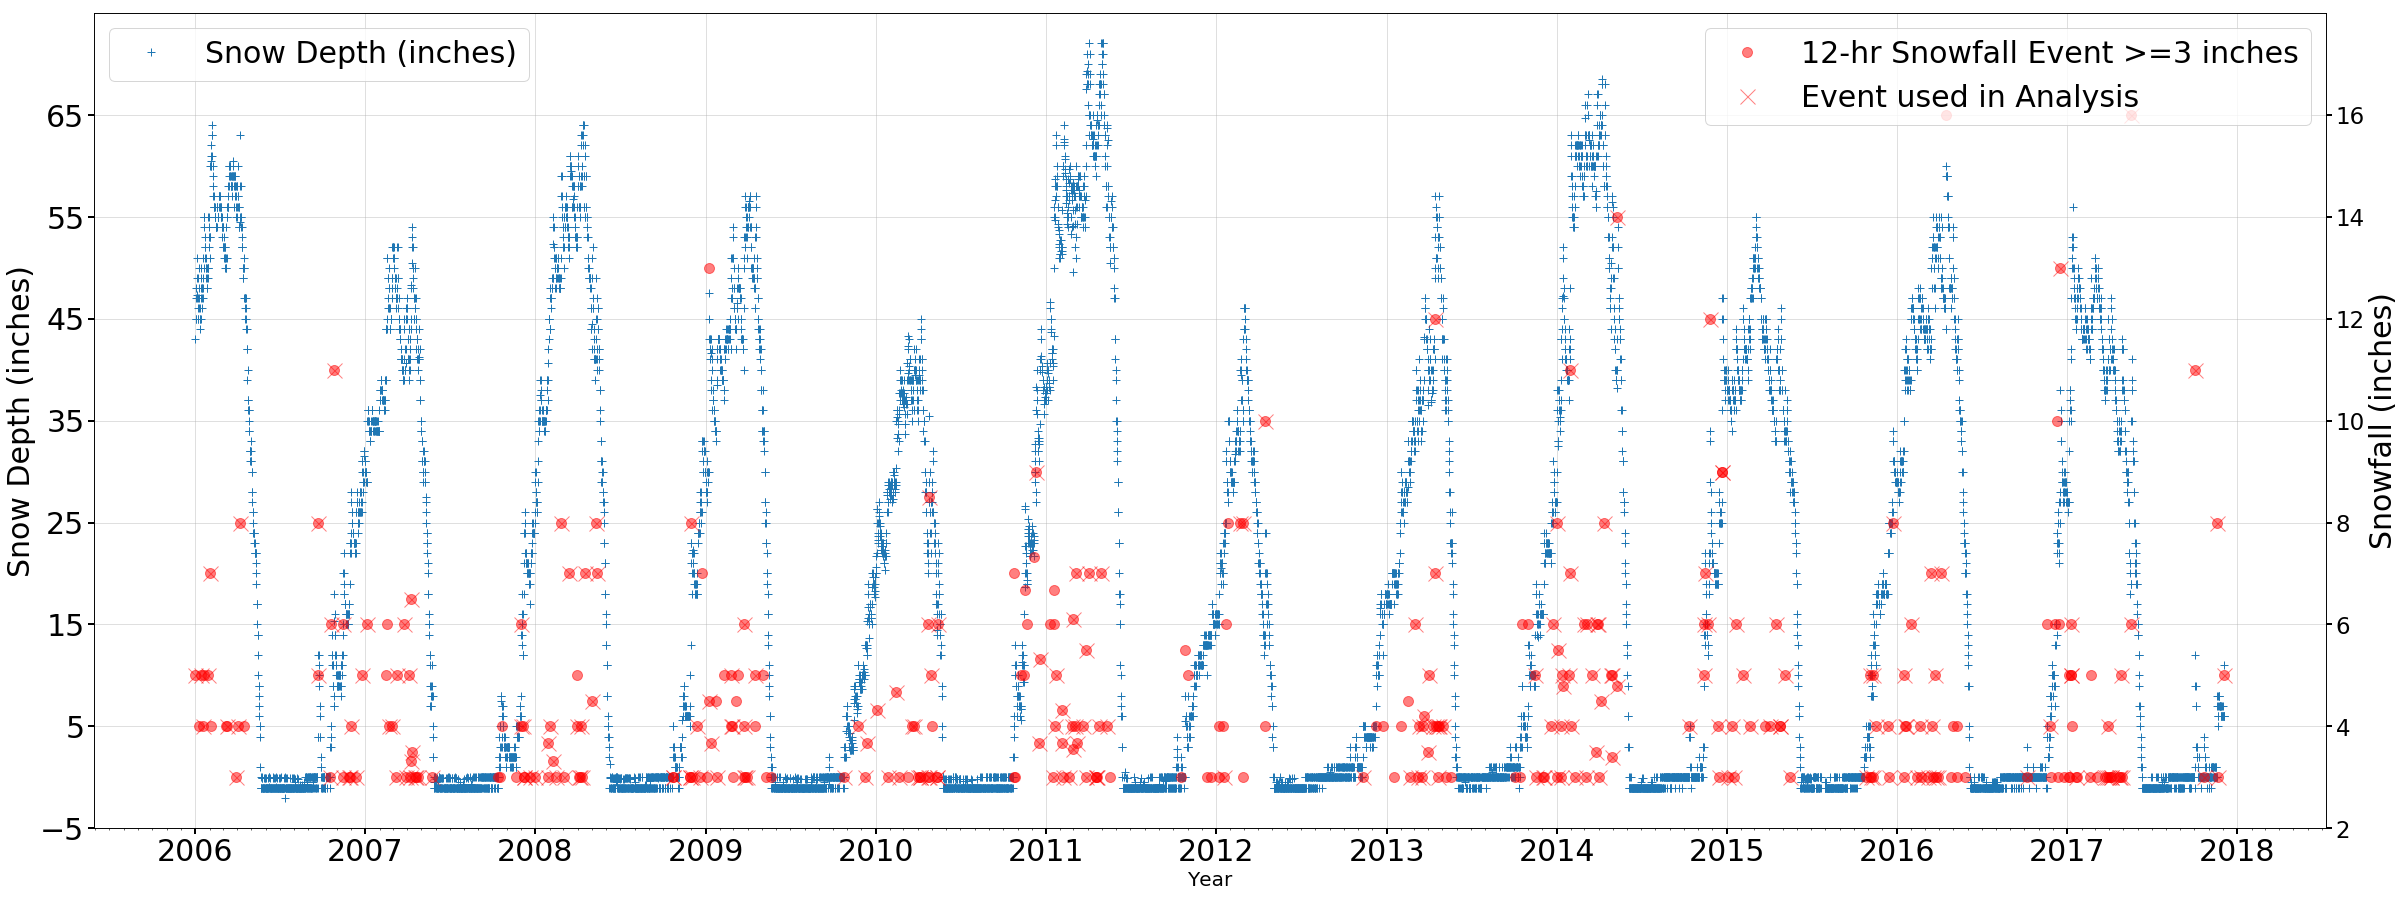
\includegraphics{https://github.com/dustinrapp/Capstone_Springboard_Intermediate_Python//Capstone/MS_CS_report/figsfigs/snowdepth_snowfall.png}
\caption{alt text}
\end{figure}

\subsection{Linear Regression
Analysis}\label{linear-regression-analysis}

To assess snowfall prediction potential with Ordinary Least Squares
model, a linear regression analysis was performed on each dataset. For
each potential variable, data was plotted against snowfall amounts which
would occur over the next 12 hours. Slope, standard error, R square
values, along with p values were calculated for all variables. A table
showing results from this analysis are shown in \textbf{Table 3}. The
data are sorted by largest R value. Note that the variables with the
best predictive capabilities are dewpoint, KCCU Wind Speed, and pressure
changes. Though Cloud Cover does have higher R values as well, the p
values and amount of data missing is also very high. While the R values
are not notably high (all are less then 0.2), p values for dewpoint,
12-hr pressure change are less then 0.05, indicating that there may be
some predictive skill with an OLS model.

\begin{center}\rule{0.5\linewidth}{\linethickness}\end{center}

\textbf{Table 3 - Output statistics from Linear Regression Analysis}

\begin{longtable}[]{@{}lllllllll@{}}
\toprule
\begin{minipage}[b]{0.25\columnwidth}\raggedright\strut
\strut
\end{minipage} & \begin{minipage}[b]{0.06\columnwidth}\raggedright\strut
Max\strut
\end{minipage} & \begin{minipage}[b]{0.06\columnwidth}\raggedright\strut
Min\footnotemark{}\strut
\end{minipage}
\footnotetext{} &
\begin{minipage}[b]{0.08\columnwidth}\raggedright\strut
Mean\footnotemark{}\strut
\end{minipage}
\footnotetext{} &
\begin{minipage}[b]{0.05\columnwidth}\raggedright\strut
Slope\strut
\end{minipage} & \begin{minipage}[b]{0.07\columnwidth}\raggedright\strut
Std Error\strut
\end{minipage} & \begin{minipage}[b]{0.06\columnwidth}\raggedright\strut
R Value\strut
\end{minipage} & \begin{minipage}[b]{0.06\columnwidth}\raggedright\strut
P-value\strut
\end{minipage} & \begin{minipage}[b]{0.07\columnwidth}\raggedright\strut
\% Missing\strut
\end{minipage}\tabularnewline
\midrule
\endhead
\begin{minipage}[t]{0.25\columnwidth}\raggedright\strut
KCCU Dewpoint (deg C)\strut
\end{minipage} & \begin{minipage}[t]{0.06\columnwidth}\raggedright\strut
0\strut
\end{minipage} & \begin{minipage}[t]{0.06\columnwidth}\raggedright\strut
-27\strut
\end{minipage} & \begin{minipage}[t]{0.08\columnwidth}\raggedright\strut
-9.7\strut
\end{minipage} & \begin{minipage}[t]{0.05\columnwidth}\raggedright\strut
0.085\strut
\end{minipage} & \begin{minipage}[t]{0.07\columnwidth}\raggedright\strut
0.03\strut
\end{minipage} & \begin{minipage}[t]{0.06\columnwidth}\raggedright\strut
0.171\strut
\end{minipage} & \begin{minipage}[t]{0.06\columnwidth}\raggedright\strut
0.005\strut
\end{minipage} & \begin{minipage}[t]{0.07\columnwidth}\raggedright\strut
21.9\strut
\end{minipage}\tabularnewline
\begin{minipage}[t]{0.25\columnwidth}\raggedright\strut
KCCU CloudCover (oktas)\strut
\end{minipage} & \begin{minipage}[t]{0.06\columnwidth}\raggedright\strut
8\strut
\end{minipage} & \begin{minipage}[t]{0.06\columnwidth}\raggedright\strut
0\strut
\end{minipage} & \begin{minipage}[t]{0.08\columnwidth}\raggedright\strut
7.4\strut
\end{minipage} & \begin{minipage}[t]{0.05\columnwidth}\raggedright\strut
0.145\strut
\end{minipage} & \begin{minipage}[t]{0.07\columnwidth}\raggedright\strut
0.085\strut
\end{minipage} & \begin{minipage}[t]{0.06\columnwidth}\raggedright\strut
0.142\strut
\end{minipage} & \begin{minipage}[t]{0.06\columnwidth}\raggedright\strut
0.089\strut
\end{minipage} & \begin{minipage}[t]{0.07\columnwidth}\raggedright\strut
57.1\strut
\end{minipage}\tabularnewline
\begin{minipage}[t]{0.25\columnwidth}\raggedright\strut
LXV Dewpoint (deg C)\strut
\end{minipage} & \begin{minipage}[t]{0.06\columnwidth}\raggedright\strut
2.8\strut
\end{minipage} & \begin{minipage}[t]{0.06\columnwidth}\raggedright\strut
-22.8\strut
\end{minipage} & \begin{minipage}[t]{0.08\columnwidth}\raggedright\strut
-8.1\strut
\end{minipage} & \begin{minipage}[t]{0.05\columnwidth}\raggedright\strut
0.074\strut
\end{minipage} & \begin{minipage}[t]{0.07\columnwidth}\raggedright\strut
0.031\strut
\end{minipage} & \begin{minipage}[t]{0.06\columnwidth}\raggedright\strut
0.134\strut
\end{minipage} & \begin{minipage}[t]{0.06\columnwidth}\raggedright\strut
0.019\strut
\end{minipage} & \begin{minipage}[t]{0.07\columnwidth}\raggedright\strut
9.5\strut
\end{minipage}\tabularnewline
\begin{minipage}[t]{0.25\columnwidth}\raggedright\strut
LXV CloudCover (oktas)\strut
\end{minipage} & \begin{minipage}[t]{0.06\columnwidth}\raggedright\strut
8\strut
\end{minipage} & \begin{minipage}[t]{0.06\columnwidth}\raggedright\strut
0\strut
\end{minipage} & \begin{minipage}[t]{0.08\columnwidth}\raggedright\strut
6.8\strut
\end{minipage} & \begin{minipage}[t]{0.05\columnwidth}\raggedright\strut
0.088\strut
\end{minipage} & \begin{minipage}[t]{0.07\columnwidth}\raggedright\strut
0.059\strut
\end{minipage} & \begin{minipage}[t]{0.06\columnwidth}\raggedright\strut
0.122\strut
\end{minipage} & \begin{minipage}[t]{0.06\columnwidth}\raggedright\strut
0.136\strut
\end{minipage} & \begin{minipage}[t]{0.07\columnwidth}\raggedright\strut
55.0\strut
\end{minipage}\tabularnewline
\begin{minipage}[t]{0.25\columnwidth}\raggedright\strut
LXV 12hr Pressure difference (hp)\strut
\end{minipage} & \begin{minipage}[t]{0.06\columnwidth}\raggedright\strut
13.35\strut
\end{minipage} & \begin{minipage}[t]{0.06\columnwidth}\raggedright\strut
-20.2\strut
\end{minipage} & \begin{minipage}[t]{0.08\columnwidth}\raggedright\strut
-3.0\strut
\end{minipage} & \begin{minipage}[t]{0.05\columnwidth}\raggedright\strut
-0.051\strut
\end{minipage} & \begin{minipage}[t]{0.07\columnwidth}\raggedright\strut
0.024\strut
\end{minipage} & \begin{minipage}[t]{0.06\columnwidth}\raggedright\strut
-0.122\strut
\end{minipage} & \begin{minipage}[t]{0.06\columnwidth}\raggedright\strut
0.033\strut
\end{minipage} & \begin{minipage}[t]{0.07\columnwidth}\raggedright\strut
10.4\strut
\end{minipage}\tabularnewline
\begin{minipage}[t]{0.25\columnwidth}\raggedright\strut
CMtn WindSpeed (m/s)\strut
\end{minipage} & \begin{minipage}[t]{0.06\columnwidth}\raggedright\strut
20.1\strut
\end{minipage} & \begin{minipage}[t]{0.06\columnwidth}\raggedright\strut
0\strut
\end{minipage} & \begin{minipage}[t]{0.08\columnwidth}\raggedright\strut
7.7\strut
\end{minipage} & \begin{minipage}[t]{0.05\columnwidth}\raggedright\strut
0.061\strut
\end{minipage} & \begin{minipage}[t]{0.07\columnwidth}\raggedright\strut
0.034\strut
\end{minipage} & \begin{minipage}[t]{0.06\columnwidth}\raggedright\strut
0.112\strut
\end{minipage} & \begin{minipage}[t]{0.06\columnwidth}\raggedright\strut
0.073\strut
\end{minipage} & \begin{minipage}[t]{0.07\columnwidth}\raggedright\strut
24.3\strut
\end{minipage}\tabularnewline
\begin{minipage}[t]{0.25\columnwidth}\raggedright\strut
CMtn Temperature (degC)\strut
\end{minipage} & \begin{minipage}[t]{0.06\columnwidth}\raggedright\strut
7\strut
\end{minipage} & \begin{minipage}[t]{0.06\columnwidth}\raggedright\strut
-21\strut
\end{minipage} & \begin{minipage}[t]{0.08\columnwidth}\raggedright\strut
-4.7\strut
\end{minipage} & \begin{minipage}[t]{0.05\columnwidth}\raggedright\strut
0.035\strut
\end{minipage} & \begin{minipage}[t]{0.07\columnwidth}\raggedright\strut
0.031\strut
\end{minipage} & \begin{minipage}[t]{0.06\columnwidth}\raggedright\strut
0.069\strut
\end{minipage} & \begin{minipage}[t]{0.06\columnwidth}\raggedright\strut
0.261\strut
\end{minipage} & \begin{minipage}[t]{0.07\columnwidth}\raggedright\strut
21.3\strut
\end{minipage}\tabularnewline
\begin{minipage}[t]{0.25\columnwidth}\raggedright\strut
CMtn Temperature (deg C)\strut
\end{minipage} & \begin{minipage}[t]{0.06\columnwidth}\raggedright\strut
7.6\strut
\end{minipage} & \begin{minipage}[t]{0.06\columnwidth}\raggedright\strut
-18.7\strut
\end{minipage} & \begin{minipage}[t]{0.08\columnwidth}\raggedright\strut
-3.6\strut
\end{minipage} & \begin{minipage}[t]{0.05\columnwidth}\raggedright\strut
0.036\strut
\end{minipage} & \begin{minipage}[t]{0.07\columnwidth}\raggedright\strut
0.03\strut
\end{minipage} & \begin{minipage}[t]{0.06\columnwidth}\raggedright\strut
0.066\strut
\end{minipage} & \begin{minipage}[t]{0.06\columnwidth}\raggedright\strut
22.6\strut
\end{minipage} & \begin{minipage}[t]{0.07\columnwidth}\raggedright\strut
0.0\strut
\end{minipage}\tabularnewline
\begin{minipage}[t]{0.25\columnwidth}\raggedright\strut
SNTL Temperature (deg C)\strut
\end{minipage} & \begin{minipage}[t]{0.06\columnwidth}\raggedright\strut
7.6\strut
\end{minipage} & \begin{minipage}[t]{0.06\columnwidth}\raggedright\strut
-18.7\strut
\end{minipage} & \begin{minipage}[t]{0.08\columnwidth}\raggedright\strut
-3.6\strut
\end{minipage} & \begin{minipage}[t]{0.05\columnwidth}\raggedright\strut
0.036\strut
\end{minipage} & \begin{minipage}[t]{0.07\columnwidth}\raggedright\strut
0.03\strut
\end{minipage} & \begin{minipage}[t]{0.06\columnwidth}\raggedright\strut
0.066\strut
\end{minipage} & \begin{minipage}[t]{0.06\columnwidth}\raggedright\strut
0.226\strut
\end{minipage} & \begin{minipage}[t]{0.07\columnwidth}\raggedright\strut
0\strut
\end{minipage}\tabularnewline
\begin{minipage}[t]{0.25\columnwidth}\raggedright\strut
LXV Temperature (deg C)\strut
\end{minipage} & \begin{minipage}[t]{0.06\columnwidth}\raggedright\strut
13.3\strut
\end{minipage} & \begin{minipage}[t]{0.06\columnwidth}\raggedright\strut
-17.2\strut
\end{minipage} & \begin{minipage}[t]{0.08\columnwidth}\raggedright\strut
-3.0\strut
\end{minipage} & \begin{minipage}[t]{0.05\columnwidth}\raggedright\strut
0.03\strut
\end{minipage} & \begin{minipage}[t]{0.07\columnwidth}\raggedright\strut
0.026\strut
\end{minipage} & \begin{minipage}[t]{0.06\columnwidth}\raggedright\strut
0.065\strut
\end{minipage} & \begin{minipage}[t]{0.06\columnwidth}\raggedright\strut
0.257\strut
\end{minipage} & \begin{minipage}[t]{0.07\columnwidth}\raggedright\strut
9.5\strut
\end{minipage}\tabularnewline
\begin{minipage}[t]{0.25\columnwidth}\raggedright\strut
LXV Wind Direction (deg)\strut
\end{minipage} & \begin{minipage}[t]{0.06\columnwidth}\raggedright\strut
360\strut
\end{minipage} & \begin{minipage}[t]{0.06\columnwidth}\raggedright\strut
0.0\strut
\end{minipage} & \begin{minipage}[t]{0.08\columnwidth}\raggedright\strut
184.1\strut
\end{minipage} & \begin{minipage}[t]{0.05\columnwidth}\raggedright\strut
-0.001\strut
\end{minipage} & \begin{minipage}[t]{0.07\columnwidth}\raggedright\strut
0.001\strut
\end{minipage} & \begin{minipage}[t]{0.06\columnwidth}\raggedright\strut
-0.055\strut
\end{minipage} & \begin{minipage}[t]{0.06\columnwidth}\raggedright\strut
0.336\strut
\end{minipage} & \begin{minipage}[t]{0.07\columnwidth}\raggedright\strut
0.095\strut
\end{minipage}\tabularnewline
\begin{minipage}[t]{0.25\columnwidth}\raggedright\strut
CMtn Wind Direction (deg)\strut
\end{minipage} & \begin{minipage}[t]{0.06\columnwidth}\raggedright\strut
360\strut
\end{minipage} & \begin{minipage}[t]{0.06\columnwidth}\raggedright\strut
0.0\strut
\end{minipage} & \begin{minipage}[t]{0.08\columnwidth}\raggedright\strut
236.5\strut
\end{minipage} & \begin{minipage}[t]{0.05\columnwidth}\raggedright\strut
0.002\strut
\end{minipage} & \begin{minipage}[t]{0.07\columnwidth}\raggedright\strut
0.002\strut
\end{minipage} & \begin{minipage}[t]{0.06\columnwidth}\raggedright\strut
0.044\strut
\end{minipage} & \begin{minipage}[t]{0.06\columnwidth}\raggedright\strut
0.48\strut
\end{minipage} & \begin{minipage}[t]{0.07\columnwidth}\raggedright\strut
0.243\strut
\end{minipage}\tabularnewline
\begin{minipage}[t]{0.25\columnwidth}\raggedright\strut
LXV Pressure (hp)\strut
\end{minipage} & \begin{minipage}[t]{0.06\columnwidth}\raggedright\strut
1028.5\strut
\end{minipage} & \begin{minipage}[t]{0.06\columnwidth}\raggedright\strut
983.3\strut
\end{minipage} & \begin{minipage}[t]{0.08\columnwidth}\raggedright\strut
1005.5\strut
\end{minipage} & \begin{minipage}[t]{0.05\columnwidth}\raggedright\strut
-0.011\strut
\end{minipage} & \begin{minipage}[t]{0.07\columnwidth}\raggedright\strut
0.015\strut
\end{minipage} & \begin{minipage}[t]{0.06\columnwidth}\raggedright\strut
-0.043\strut
\end{minipage} & \begin{minipage}[t]{0.06\columnwidth}\raggedright\strut
0.457\strut
\end{minipage} & \begin{minipage}[t]{0.07\columnwidth}\raggedright\strut
10.1\strut
\end{minipage}\tabularnewline
\begin{minipage}[t]{0.25\columnwidth}\raggedright\strut
LXV WindSpeed m/s\strut
\end{minipage} & \begin{minipage}[t]{0.06\columnwidth}\raggedright\strut
13.4\strut
\end{minipage} & \begin{minipage}[t]{0.06\columnwidth}\raggedright\strut
0.0\strut
\end{minipage} & \begin{minipage}[t]{0.08\columnwidth}\raggedright\strut
3.7\strut
\end{minipage} & \begin{minipage}[t]{0.05\columnwidth}\raggedright\strut
0.005\strut
\end{minipage} & \begin{minipage}[t]{0.07\columnwidth}\raggedright\strut
0.054\strut
\end{minipage} & \begin{minipage}[t]{0.06\columnwidth}\raggedright\strut
0.005\strut
\end{minipage} & \begin{minipage}[t]{0.06\columnwidth}\raggedright\strut
0.926\strut
\end{minipage} & \begin{minipage}[t]{0.07\columnwidth}\raggedright\strut
9.5\strut
\end{minipage}\tabularnewline
\bottomrule
\end{longtable}

\subsection{Conclusion}\label{conclusion}

While not large, there are some significant relationships between some
meteorological variables and snowfall amount when snowfall does occur.
It is anticipated that there may be some 12-hr snowfall predictive
ability predicting snowfall utilizing a very simple Ordinary Least
Squares model with these meteorological measurements. Additional data
sources, such as upper air measurements could be utilized to improve
predictive ability.


    % Add a bibliography block to the postdoc
    
    
    
    \end{document}
